\chapter{Bayes classifier}

{\sf Bayes classifier is actually straight forward thing and really easy to understand and to implement. It is one of the most used method in text classification (for example, spam mail detection). We use Bayes classifier if our feature space is more than our dataset and it is proved to be optimal. In this lecture we will talk about naive Bayes classifier (what assume that all features are independent). Also there are Bayes optimal classifier (method for combining classifiers) and Bayes optimization (how to optimize the hyperparameters of our classifier or smth else). However Bayes optimal classifier is not used at all, Bayes optimization is used sometimes; Bayes methods in Deep Learning are not used at all except research.}

\section{Naive Bayes Classifier}

In Bayes classifiers we try to calculate the probability that the point $x$ belongs to the class $y$:
$$P(y|x)=\frac{P(y)P(x|y)}{P(x)}$$
So we say that the class of $x$ will be $y_{MAP}$ (MAP is a Maximal Apostriority Probability):
$$y_{MAP}=\arg\max\limits_{y\in Y} P(y|x)=\arg\max\limits_{y\in Y}\frac{P(y)P(x|y)}{P(x)}=\arg\max\limits_{y\in Y} P(y)P(x|y);$$
$$\arg\max\limits_{y\in Y} P(y)P(x|y)=\arg\max\limits_{y\in Y} P(x_1,\ldots,x_n|y)P(y);$$
where $x_1,\ldots,x_n$ are features of point $x$. $P(y)$ is a frequency of class $y$ in our dateset. In naive assumption (when features are independent) we have
$$P(x_1,\ldots,x_n|y)=P(x_1|y)\cdot\ldots\cdot P(x_n|y);$$
$$P(x_i|y)=\frac{count(x_i,y)}{count(y)};$$
[$count(x_i, y)$ -- количество точек из класса $y$ в нашем датасете, у которых $i$-ая фича равна $x_i$, $count(y)$ -- количество всех точек в классе $y$.] To avoid case $count(x_i,y_i)=0$ we assume that there are at least $\alpha$ points of each class with feature $x_i$:
$$P (x_i|y)=\frac{count(x_i,y)+\alpha}{count(y)+\alpha K}$$
where $K$ is the number of classes.

\subsubsection*{Bag of words}

The main application area of naive Bayes classifier is text because there are so many features. But we just calculate the word frequences in the text using bag of words. And the features of the text are just the numbers of some words in it.

\subsubsection*{Examples of Bayes classifiers with various types of features}

Binary features:
$$P(x_i|y)=P(x_1=1|y)x_i+(1-P(x_i=1|y))(1-x_i),\qquad x_i\in\{0,1\}$$
Continious features (normal distribution):
$$p(x_i|y)=\frac{1}{\sqrt{2\pi\sigma_y^2}}\cdot e^{-(x_i-\mu_y)^2/2\sigma_y^2}$$
where $\mu_y$ and $\sigma_y$ are some parameters of distribution for a class $y$. \\
If the features distributed not by the normal distribution, we can approximate it by the mixture of normal distributions. In this case we use expectation-maximization (EM) algorithm.

\section{Expectation-Maximization Algorithm}

So we have $K$ multidimensional normal distributions and each of them defined by:
\begin{enumerate}[label=$\bullet$]
	\item $\mu_k$ -- mean vector,
	\item $\sigma_k$ -- covariance matrix,
	\item $\alpha_k$ -- weight of distribution $k$, a probability that random point belongs to it ($\sum\alpha_k=1$).
\end{enumerate}
How we find optimal parameters of distributions? We use E-Step and the M-Step. E-Step is calculating $w_{ik}$ -- affinity of point $x_i$ to distribution $k$:
$$w_{ik} = p(\mu_k,\sigma_k|x_i)=\frac{p(x_i|\mu_k,\sigma_k)\cdot\alpha_k}{\sum\limits_{j=1}^{K}p(x_i|\mu_j,\sigma_j)\cdot\alpha_j};$$
$$p(x_i|\mu_k, \sigma_k)=\frac{1}{\sqrt{2\pi\sigma_k^2}}\cdot e^{-(x_i-\mu_k)^2/2\sigma_k^2};$$
First E-Step chooses distributions parameters randomly.\\
M-Step is recalculating all parameters:
$$\begin{cases}
	a_k^{new}=\frac{1}{N}\sum\limits_{i=1}^{N}w_{ik}=\frac{N_k}{N} \\
	\mu_k^{new}=\frac{1}{N_k}\sum\limits_{i=1}^{N}w_{ik}x_i \\
	\sigma_k^{new}=\frac{1}{N_k}\sum\limits_{i=1}^{N}w_{ik}(x_i-\mu_k^{new})(x_i-\mu_k^{new})^T
\end{cases}$$
How it works in practise?

\subsubsection*{EM Clustering}

Let's imagine we want to unite points in two clusters. We can assume that point of each cluster distributed by the normal distribution. So the steps of EM algorithm looks like this:\\
\begin{figure}[H]
  \centering
  \begin{tabular}{ccc}
    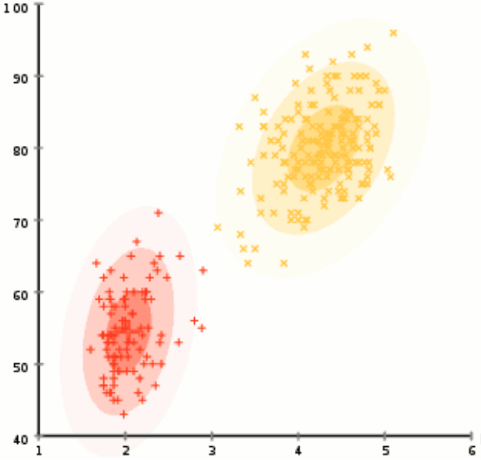
\includegraphics[width=0.25\linewidth]{10a.png} & \hspace{0.5cm}
    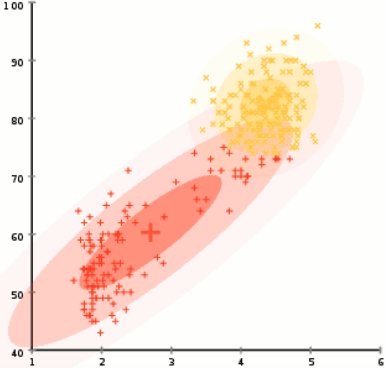
\includegraphics[width=0.25\linewidth]{10b.png} & \hspace{0.5cm}
    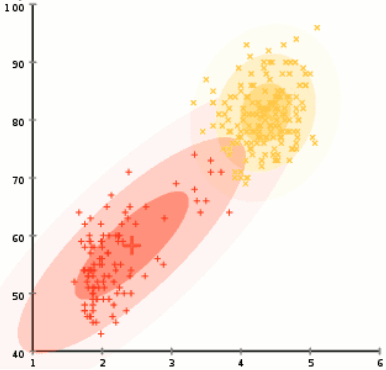
\includegraphics[width=0.25\linewidth]{10c.png} \\
    Step 1 & Step 2 & Step 3 \\
    & & \\
    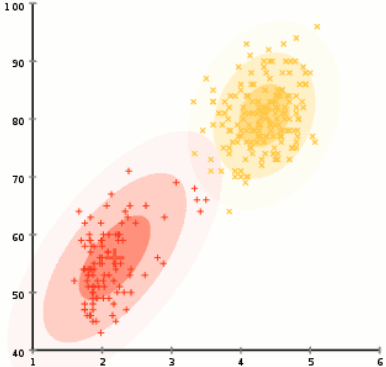
\includegraphics[width=0.25\linewidth]{10d.png} & \hspace{0.5cm}
    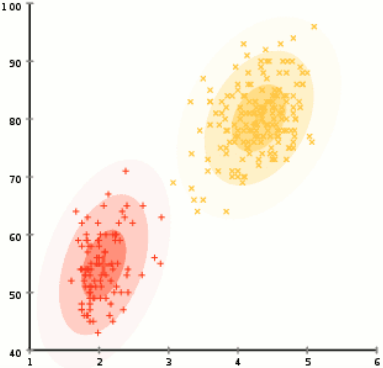
\includegraphics[width=0.25\linewidth]{10e.png} & \hspace{0.5cm}
    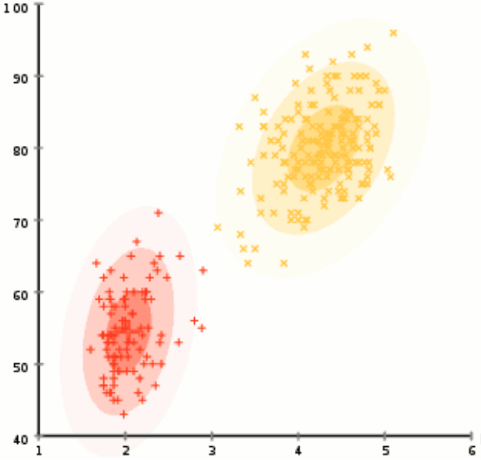
\includegraphics[width=0.25\linewidth]{10f.png} \\
    Step 4 & Step 5 & Step 6 \\
  \end{tabular}
\end{figure}

\subsubsection*{Naive Bayes is a very nice baseline!}

Naive Bayes is a very nice baseline! When you approach a new data task and collect the data, you may find that some complex algorithms don't work. And you don't know: is it a problem with data or with chosen algorithm? So you need a baseline -- something that almost always works. In that case naive Bayes can help you.